\documentclass[10pt,a4paper]{article}
\usepackage[utf8]{inputenc}
\usepackage[spanish]{babel}
\usepackage{amsmath}
\usepackage{amsfonts}
\usepackage{amssymb}
\usepackage{graphicx}
\usepackage{hyperref}
\pagenumbering{gobble}
\usepackage[left=1cm,right=1cm,top=1cm,bottom=1cm]{geometry}


\title{Summary of ``\textit{Xception}: Deep Learning with Depthwise Separable Convolutions''}
\date{\vspace{-5ex}}
\author{Iván Vallés Pérez}

\begin{document}
\maketitle

\begin{description}
	\item[Title]: \textit{Xception}: Deep Learning with Depthwise Separable Convolutions
	\item[Authors]: François Chollet
	\item[Journal]: Google report
	\item[Date]: April 2017
\end{description}

\section*{Convolution vs depthwise separable convolution\footnote{Material borrowed from here \url{https://www.youtube.com/watch?v=T7o3xvJLuHk&t=337s}}}
Given an input tensor of shape (1, $D_F$, $D_F$, $M$), we are interested in applying a convolutional operation producing an output tensor of shape (1, $D_G$, $D_G$, $N$)

\subsection*{Convolution}
A convolutional layer consists of $N$ kernels with size $D_K$. In order to perform this calculation, the number of needed operations are: $M \cdot D_K^2 \cdot D_G^2 \cdot N$

\begin{figure}[h!]
	\centering
	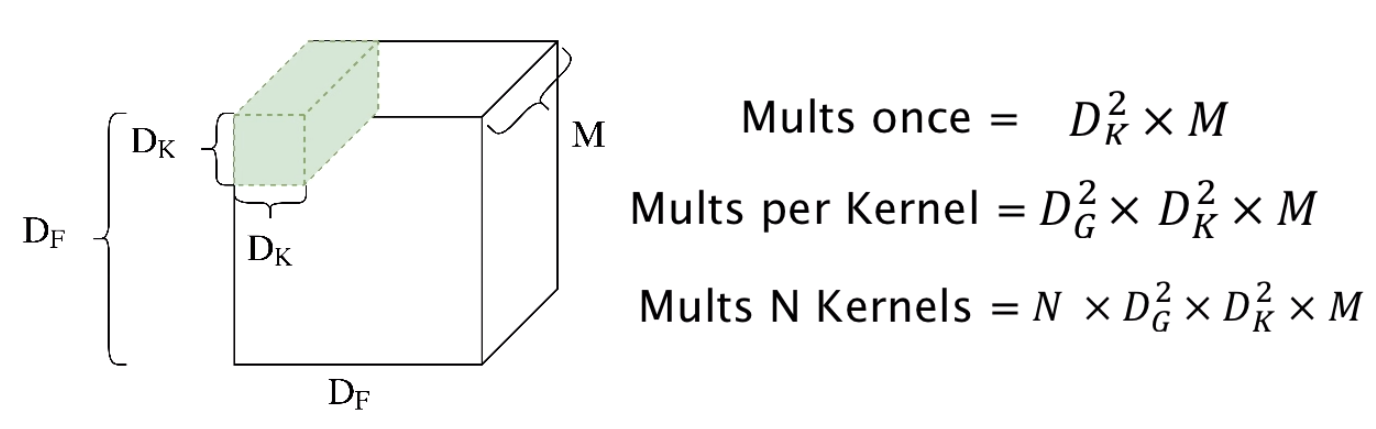
\includegraphics[width=0.4\textwidth]{img/conv_ops.png}
\end{figure}

\subsection*{Depthwise separable convolution}

\begin{enumerate}
\item Filtering stage: performed using the depthwise convolution operation. This operation consists of applying $M$ convolutions of $D_K$ size, separatedly (one for each channel); instead of one for all the channels. I.e. for each channel, only one different kernel is used. This operation produces an output tensor of shape (1, $D_G$, $D_G$, $M$). The number of needed operations at this stage is $M \cdot D_K^2 \cdot D_G^2$.
\begin{figure}[h!]
	\centering
	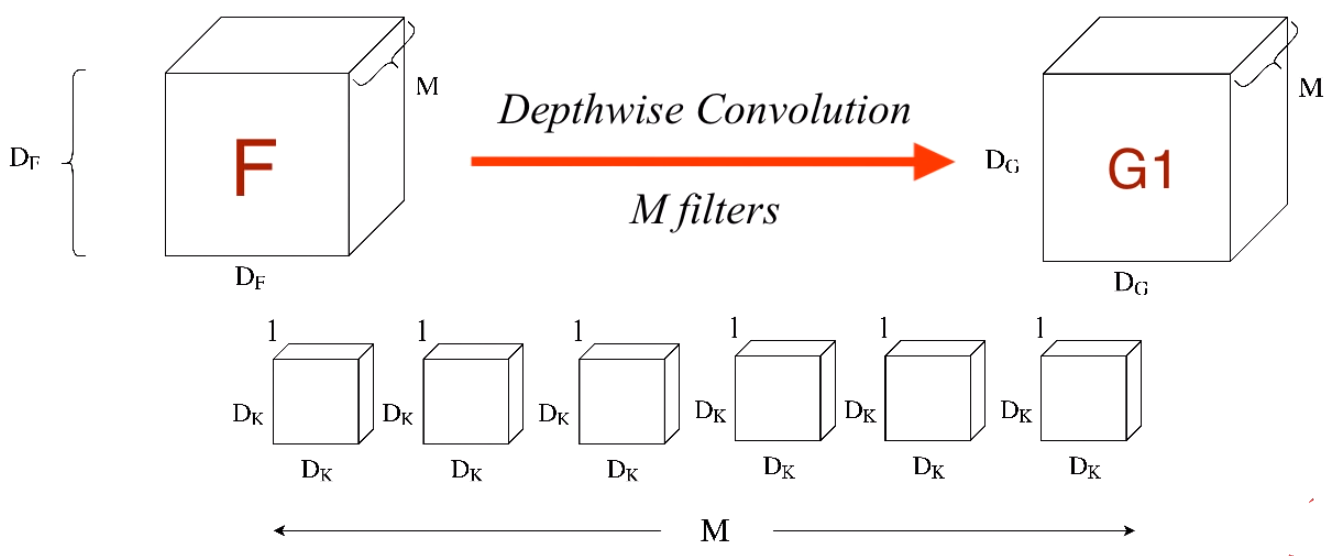
\includegraphics[width=0.4\textwidth]{img/dw_conv.png}
\end{figure}
\item Combining stage: performed using the pointwise convolution operation. This operation consists of a set of $N$ size 1 convolutions applied over the output of the previous step, leading to a tensor of shape (1, $D_G$, $D_G$, $N$). The number of needed operations at this stage is then $M \cdot D_G^2 \cdot N$
\begin{figure}[h!]
	\centering
	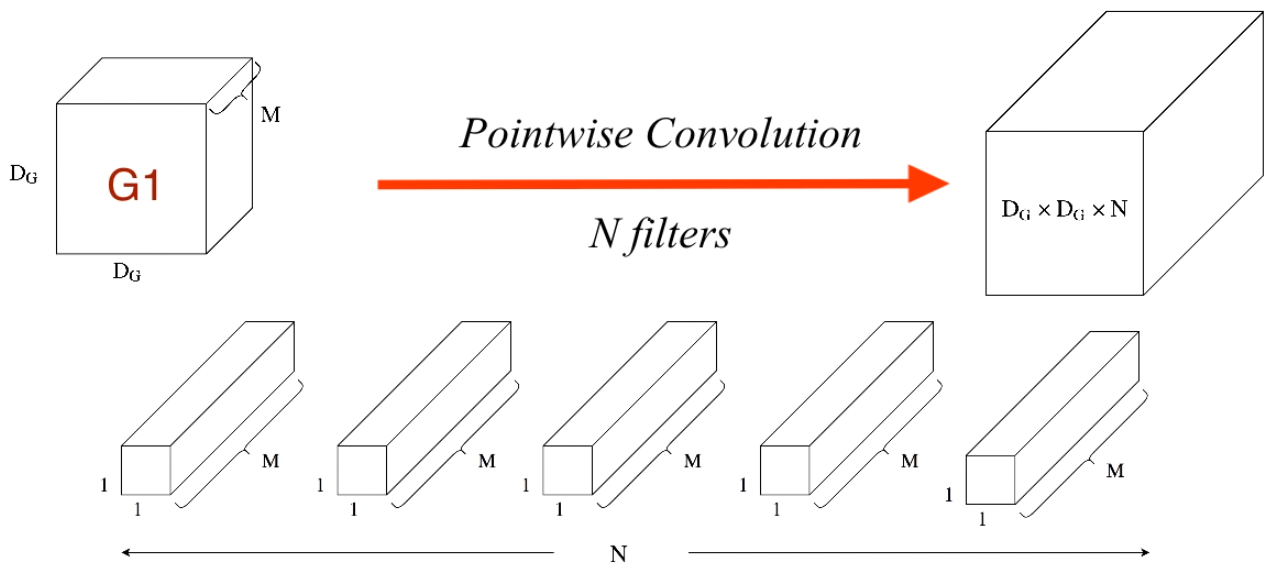
\includegraphics[width=0.4\textwidth]{img/pw_conv.png}
\end{figure}
\end{enumerate} 




The total operations performed in the depthwise separable convolution layer sums to $M \cdot D_K^2 \cdot D_G^2 + M \cdot D_G^2 \cdot N$, which reduces to $M \cdot D_G^2 \cdot \left(D_K^2 + N\right)$. This is $\frac{1}{N}\cdot\frac{1}{D_K^2}$ times the operations needed by the standard convolution. 

\section*{\textit{Xception} architecture}
\begin{itemize}
\item The main goal of the paper is to compare \textit{Inception} V3 with a \textit{Xception} architecture with similar number of parameters to see which one performs the best.
\item The \textit{Xception} is inspired in the \textit{Inception} architecture which achieved a much more efficient usage of the parameters of the network (less operations with better performance).
\item The \textit{Xception} algorithm exploits the deepthwise separable convolutions to reduce the number of operations needed in each step.
\item One difference between \textit{Xception} and \textit{Inception} is the order of operations: \textit{Xception} applies a 1x1 convolution as a final operation (pointwise convolution) while \textit{Inception} applies it at the begining. 
\item Another important difference between \textit{Xception} and \textit{Inception} is that in \textit{Inception}, each of the convolutions are followed by a non-linearity while in \textit{Xception} not including non-linearities between depthwise and pointwise convolutions showed better performance.
\item The last but not less important difference is the addition of skip connections in the \textit{Xception} architecture.
\item The main hypothesis being tested in this paper is that the mapping of cross-channels correlations and spatial correlations in the feature maps of convolutional neural networks can be entirely decoupled. As it is a stronger hypothesis than the one tested in the \textit{Inception} algorithm, the author decided to call it \textit{Xception} (extreme \textit{Inception}).
\item In short, the \textit{Xception} architecture is a linear stack of depthwise separable convolution layers with residual connections. The full architecture is described in the image below (borrowed from the original paper), in which all Convolution and SeparableConvolution layers are followed by batch normalization, even if it is not included in the diagram.
\end{itemize}

\begin{figure}[h!]
	\centering
	\includegraphics[width=0.5\textwidth]{img/Xception_architecture.png}
\end{figure}

\section*{Results and conclusions}
Both architectures were tested over two datasets. The \textit{Xception} architecture achieved a significantly better performance without tunning the architecture to each specific problem.

\begin{itemize}
\item The residual connections (or skip connections) showed to be a key element for the high performance obtained.
\item Intermediate activations in the depthwise separable layers have been tested leading to a worse result.
\item The autor concludes with a recommendation: replace \textit{Inception} modules by depthwise separable convolutions, in neural computer vision architectures.
\end{itemize}

\begin{figure}[h!]
	\centering
	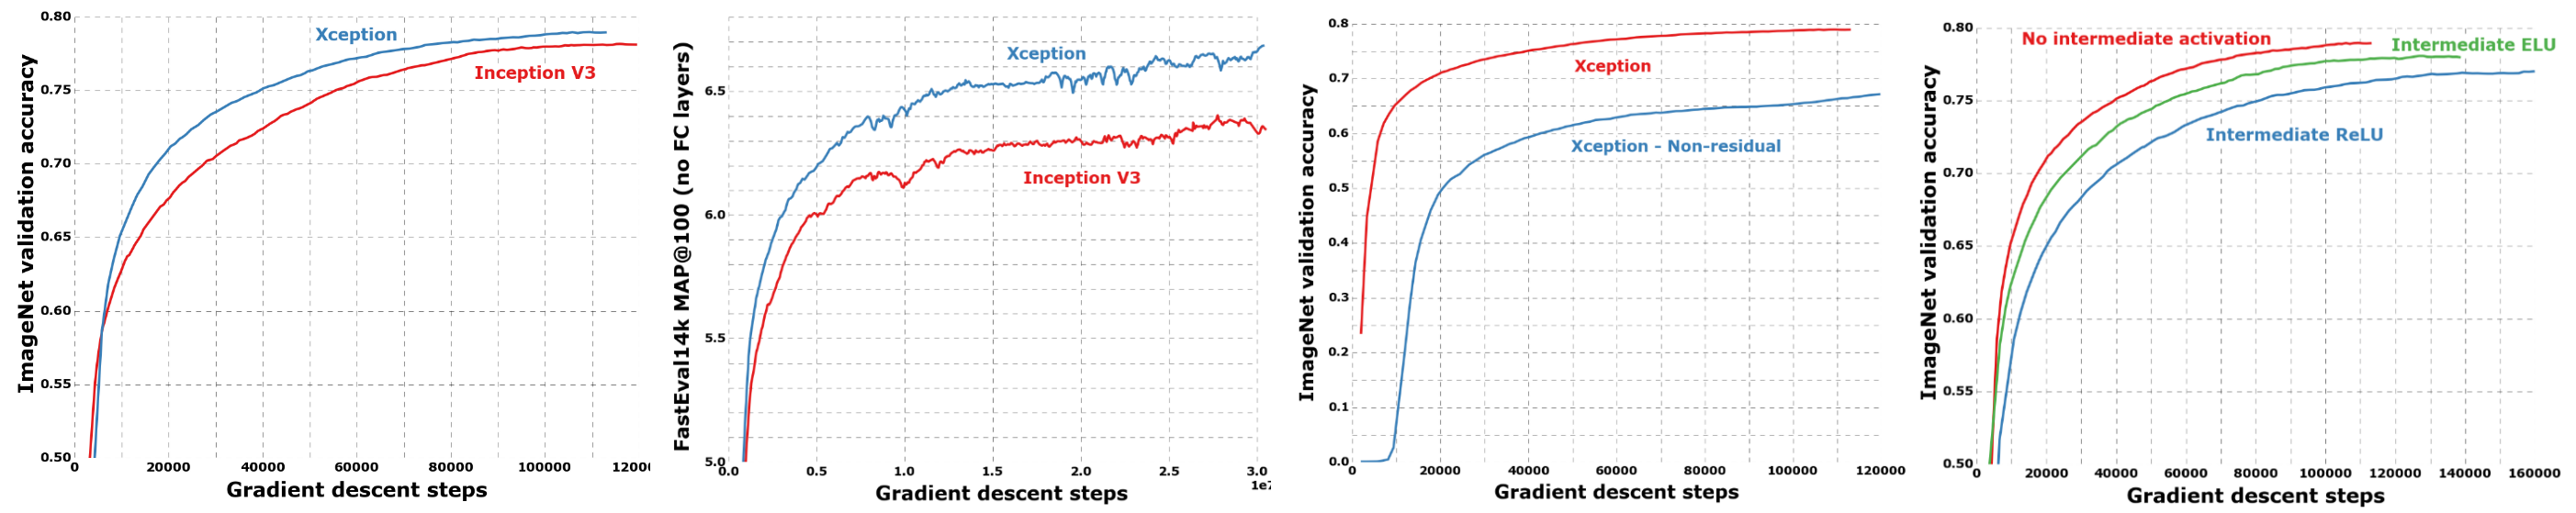
\includegraphics[width=0.9\textwidth]{img/results.png}
\end{figure}

\end{document}